\documentclass[tikz,border=10pt]{standalone}
\usepackage{tikz}
\usetikzlibrary{positioning,arrows.meta,calc,fit,backgrounds}

\definecolor{basecolor}{RGB}{30,90,160}
\definecolor{reprcolor}{RGB}{30,120,60}
\definecolor{rlcolor}{RGB}{160,80,20}
\definecolor{goalcolor}{RGB}{100,30,130}
\definecolor{loopcolor}{RGB}{20,110,130}

\tikzset{
  base/.style={
    draw=basecolor,
    fill=basecolor!10,
    rounded corners=4pt,
    minimum width=7cm,
    align=center,
    font=\bfseries,
    inner sep=8pt
  },
  tracktitle/.style={
    font=\small\bfseries,
    align=center
  },
  aebox/.style={
    draw=reprcolor,
    fill=reprcolor!8,
    rounded corners=3pt,
    text width=2cm,
    minimum height=3cm,
    align=center,
    font=\small,
    inner sep=5pt
  },
  loopbox/.style={
    draw=loopcolor,
    fill=loopcolor!8,
    rounded corners=4pt,
    text width=7cm,
    align=left,
    font=\small,
    inner sep=10pt
  },
  rlbranch_dpo/.style={
    draw=rlcolor,
    fill=rlcolor!8,
    rounded corners=3pt,
    text width=2cm,
    minimum height=3cm,
    align=center,
    font=\small,
    inner sep=6pt
  },
  rlbranch_rl/.style={
    draw=rlcolor,
    fill=rlcolor!8,
    rounded corners=3pt,
    text width=3cm,
    minimum height=1.2cm,
    align=center,
    font=\small,
    inner sep=6pt
  },
  prodbox/.style={
    draw=reprcolor,
    fill=reprcolor!12,
    rounded corners=4pt,
    text width=7cm,
    align=center,
    font=\small\bfseries,
    inner sep=8pt
  },
  splitbox/.style={
    draw=reprcolor,
    fill=reprcolor!8,
    rounded corners=3pt,
    text width=2cm,
    minimum height=2cm,
    align=center,
    font=\small,
    inner sep=6pt
  },
  goalbox/.style={
    draw=goalcolor,
    fill=goalcolor!10,
    rounded corners=4pt,
    minimum width=7cm,
    align=center,
    font=\bfseries,
    inner sep=10pt
  },
  arr/.style={
    -{Stealth[length=6pt]},
    thick
  },
  line/.style={
    thick
  }
}

\begin{document}

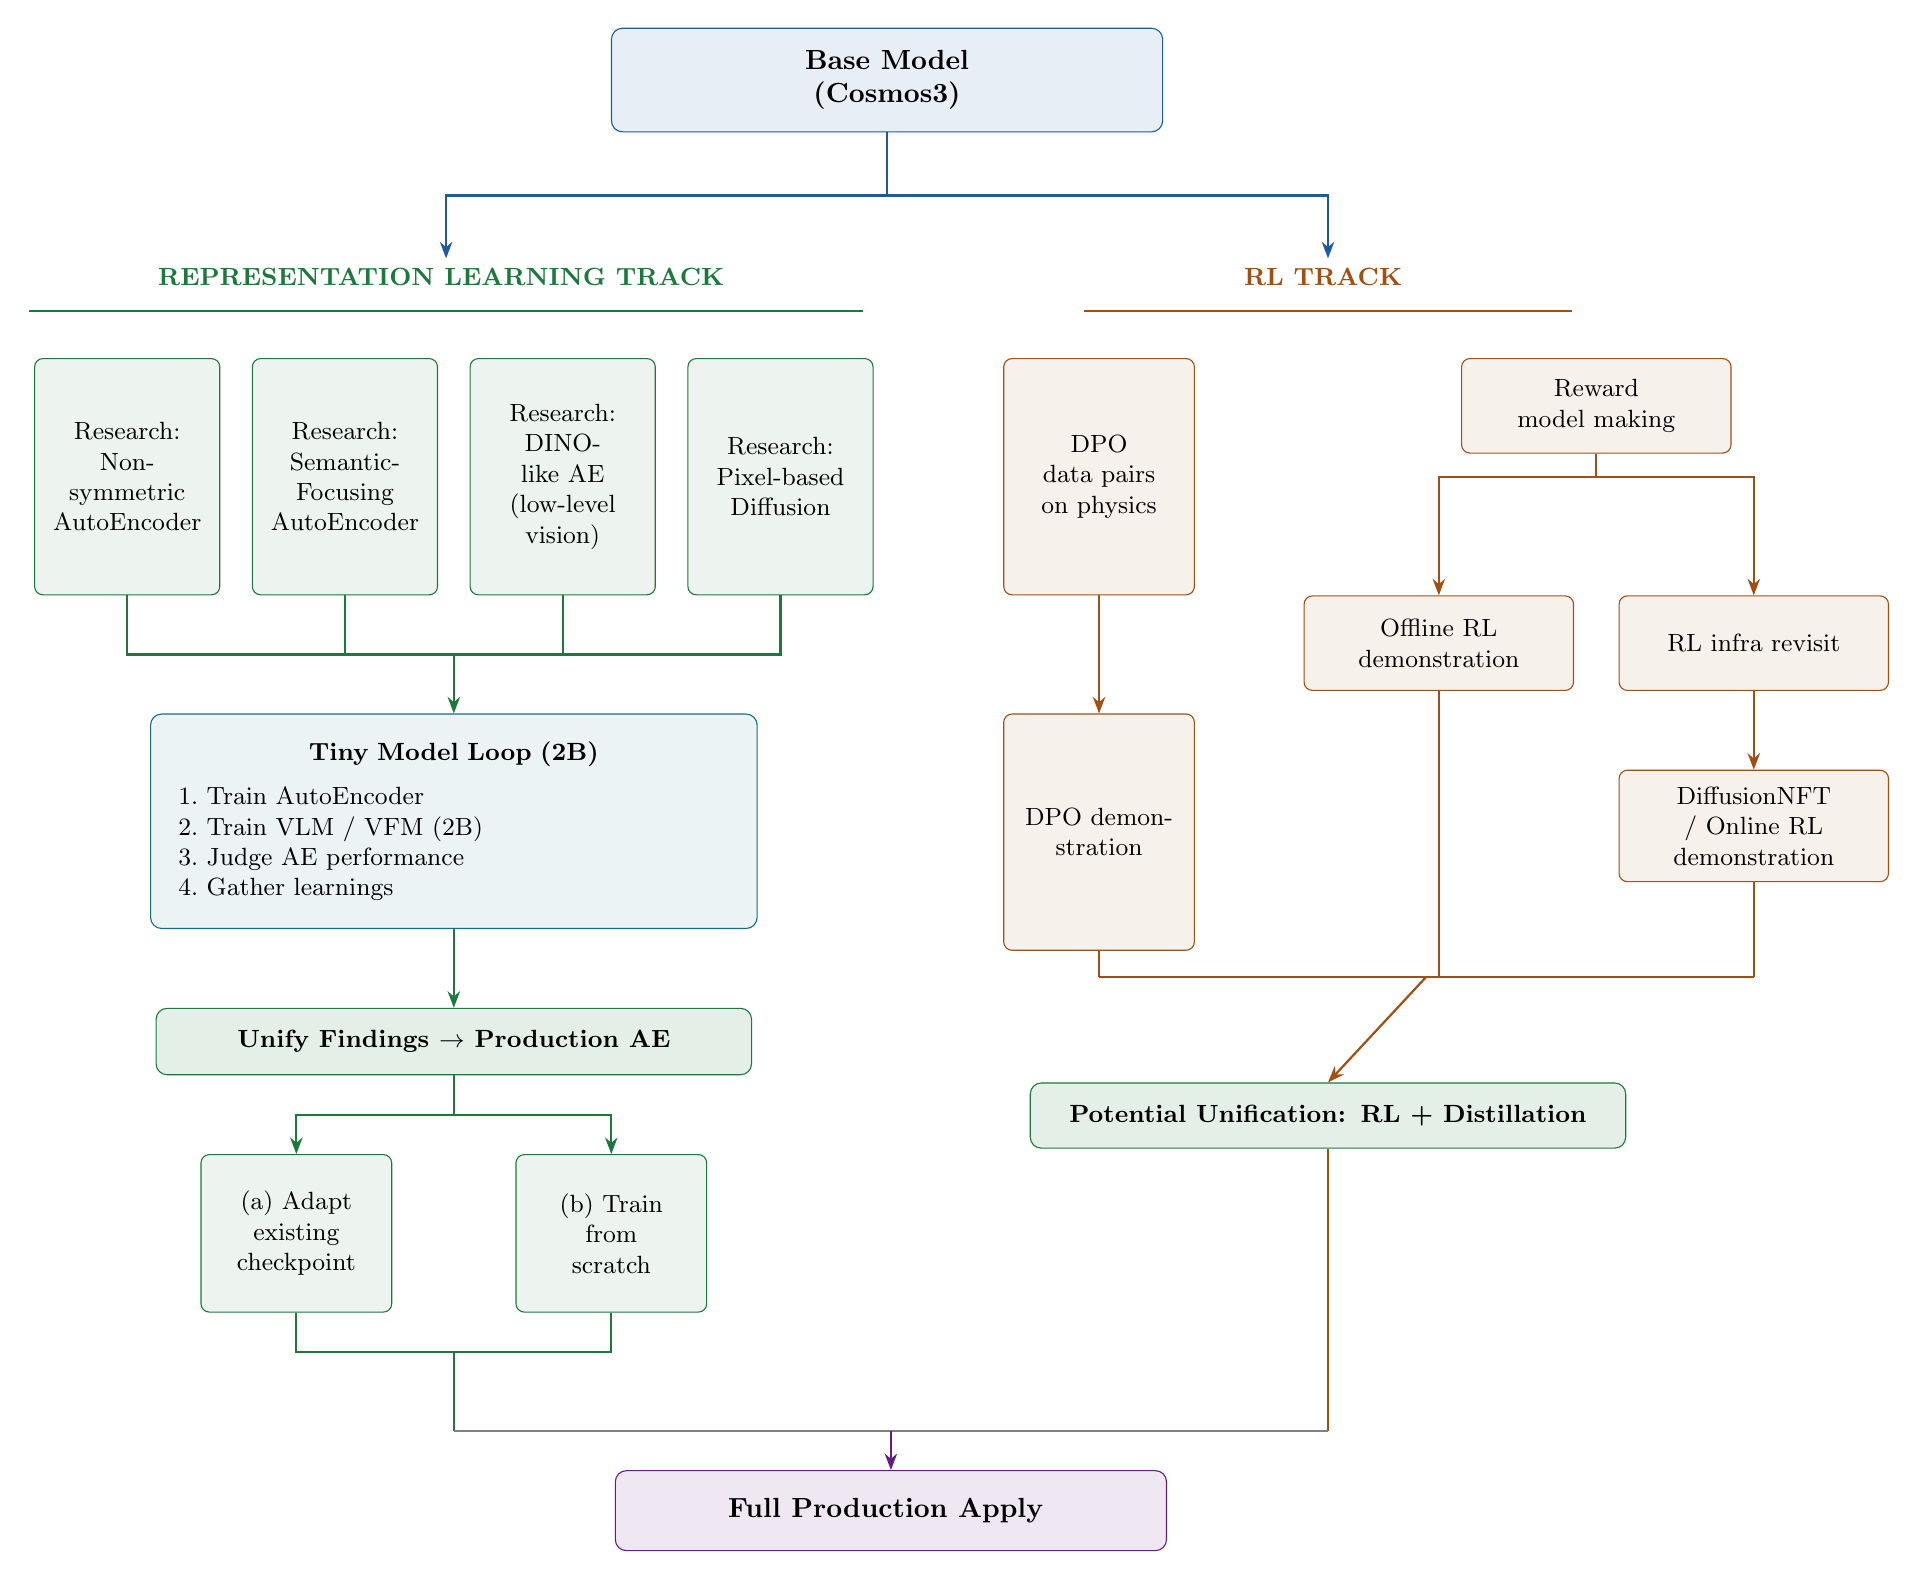
\begin{tikzpicture}[node distance=6mm and 10mm]

% ---------------------------------------------------------------------------
% Base model
% ---------------------------------------------------------------------------

\node[base] (base) {
  Base Model\\
  (Cosmos3)
};

% ---------------------------------------------------------------------------
% Track titles
% ---------------------------------------------------------------------------

\node[
  tracktitle,
  text=reprcolor,
  below=16mm of base,
  xshift=-5.6cm
] (reprtitle) {
  REPRESENTATION LEARNING TRACK
};

\node[
  tracktitle,
  text=rlcolor,
  below=16mm of base,
  xshift=5.6cm
] (rltitle) {
  RL TRACK
};

% Horizontal rules below track titles

\coordinate (reprruleL)
  at ([xshift=-5.3cm,yshift=-2mm]reprtitle.south);

\coordinate (reprruleR)
  at ([xshift=5.3cm,yshift=-2mm]reprtitle.south);

\coordinate (rlruleL)
  at ([xshift=-3.1cm,yshift=-2mm]rltitle.south);

\coordinate (rlruleR)
  at ([xshift=3.1cm,yshift=-2mm]rltitle.south);

\draw[line,reprcolor] (reprruleL) -- (reprruleR);
\draw[line,rlcolor]   (rlruleL)   -- (rlruleR);

% ---------------------------------------------------------------------------
% Representation-learning experiments
% ---------------------------------------------------------------------------

\node[
  aebox,
  below=8mm of reprtitle,
  xshift=-4.05cm
] (ae1) {
  Research:
  Non-symmetric\\
  AutoEncoder
};

\node[aebox,right=4mm of ae1] (ae2) {
  Research:
  Semantic-Focusing\\
  AutoEncoder
};

\node[aebox,right=4mm of ae2] (ae3) {
  Research:
  DINO-like AE\\
  (low-level vision)
};

\node[aebox,right=4mm of ae3] (ae4) {
  Research:
  Pixel-based\\
  Diffusion
};

% ---------------------------------------------------------------------------
% Tiny-model loop
% ---------------------------------------------------------------------------

\node[
  loopbox,
  below=15mm of $(ae2.south)!0.5!(ae3.south)$
] (loop) {
  \centering
  \textbf{Tiny Model Loop (2B)}
  \\[5pt]
  \raggedright
  1.\ Train AutoEncoder\\
  2.\ Train VLM / VFM (2B)\\
  3.\ Judge AE performance\\
  4.\ Gather learnings
};

% ---------------------------------------------------------------------------
% Production AE
% ---------------------------------------------------------------------------

\node[prodbox,below=10mm of loop] (prodae) {
  Unify Findings $\rightarrow$ Production AE
};

\node[
  splitbox,
  below=10mm of prodae,
  xshift=-2cm,
] (adapt) {
  (a) Adapt existing\\
  checkpoint
};

\node[
  splitbox,
  below=10mm of prodae,
  xshift=2cm,
] (scratch) {
  (b) Train from\\
  scratch
};

% ---------------------------------------------------------------------------
% RL chain
% ---------------------------------------------------------------------------

% Left branch: DPO
\node[rlbranch_dpo, below left=8mm and 5mm of rltitle] (rl_dpo_data) {
  DPO data pairs\\on physics
};
\node[rlbranch_dpo, below=15mm of rl_dpo_data] (rl_dpo_demo) {
  DPO demonstration
};

% Right branch: Reward model + downstream
\node[rlbranch_rl, below right=8mm and 5mm of rltitle] (rl_reward) {
  Reward model making
};
\node[rlbranch_rl, below=18mm of rl_reward, xshift=-20mm] (rl_offline) {
  Offline RL demonstration
};
\node[rlbranch_rl, below=18mm of rl_reward, xshift=20mm] (rl_infra) {
  RL infra revisit
};
\node[rlbranch_rl, below=10mm of rl_infra] (rl_online) {
  DiffusionNFT / Online RL demonstration
};

% Unification: merges both RL branches, centered under rltitle
\node[prodbox, below=100mm of rltitle] (rl_unify) {
  Potential Unification: RL + Distillation
};

% ---------------------------------------------------------------------------
% Base model to track split
% ---------------------------------------------------------------------------

\coordinate (basesplit) at ([yshift=-8mm]base.south);

\draw[line,basecolor]
  (base.south) -- (basesplit);

\draw[arr,basecolor]
  (basesplit) -| (reprtitle.north);

\draw[arr,basecolor]
  (basesplit) -| (rltitle.north);

% ---------------------------------------------------------------------------
% AE experiment boxes converge into loop
% ---------------------------------------------------------------------------

\coordinate (aejoin)
  at ([yshift=-7.5mm]$(ae2.south)!0.5!(ae3.south)$);

\foreach \boxname in {ae1,ae2,ae3,ae4}{
  \draw[line,reprcolor]
    (\boxname.south)
    -- ++(0,-7.5mm)
    -| (aejoin);
}

\draw[arr,reprcolor]
  (aejoin) -- (loop.north);

% ---------------------------------------------------------------------------
% Representation-learning flow
% ---------------------------------------------------------------------------

\draw[arr,reprcolor]
  (loop.south) -- (prodae.north);

\draw[arr,reprcolor]
  (prodae.south)
  -- ++(0,-5mm)
  -| (adapt.north);

\draw[arr,reprcolor]
  (prodae.south)
  -- ++(0,-5mm)
  -| (scratch.north);

% ---------------------------------------------------------------------------
% RL flow
% ---------------------------------------------------------------------------

% Left branch flow
\draw[arr, rlcolor] (rl_dpo_data.south) -- (rl_dpo_demo.north);

% Right branch: rl_reward splits into rl_offline and rl_infra (parallel)
\coordinate (rightSubSplit) at ([yshift=-3mm]rl_reward.south);
\draw[line, rlcolor] (rl_reward.south) -- (rightSubSplit);
\draw[arr,  rlcolor] (rightSubSplit) -| (rl_offline.north);
\draw[arr,  rlcolor] (rightSubSplit) -| (rl_infra.north);

% rl_infra connects sequentially down to rl_online
\draw[arr, rlcolor] (rl_infra.south) -- (rl_online.north);

% Single merge bar: rl_dpo_demo + rl_offline + rl_online all feed rl_unify
\coordinate (rlmergeLevel) at ([yshift=-12mm]rl_online.south);
\coordinate (rlmergeL) at (rl_dpo_demo.south |- rlmergeLevel);
\coordinate (rlmergeM) at (rl_offline.south  |- rlmergeLevel);
\coordinate (rlmergeR) at (rl_online.south   |- rlmergeLevel);

\draw[line, rlcolor] (rl_dpo_demo.south) -- (rlmergeL);
\draw[line, rlcolor] (rl_offline.south)  -- (rlmergeM);
\draw[line, rlcolor] (rl_online.south)   -- (rlmergeR);
\draw[line, rlcolor] (rlmergeL)          -- (rlmergeR);
\draw[arr,  rlcolor] ($(rlmergeL)!0.5!(rlmergeR)$) -- (rl_unify.north);

% ---------------------------------------------------------------------------
% Merge representation branches
% ---------------------------------------------------------------------------

\coordinate (reprmerge)
  at ([yshift=-10mm]$(adapt.south)!0.5!(scratch.south)$);

\draw[line,reprcolor]
  (adapt.south)
  -- ++(0,-5mm)
  -| (reprmerge);

\draw[line,reprcolor]
  (scratch.south)
  -- ++(0,-5mm)
  -| (reprmerge);

% ---------------------------------------------------------------------------
% Merge representation and RL tracks
% ---------------------------------------------------------------------------

\coordinate (mergeL)
  at ([yshift=-5mm]reprmerge);

\coordinate (mergeR)
  at (rltitle.center |- mergeL);

\coordinate (finalmerge)
  at ($(mergeL)!0.5!(mergeR)$);

\draw[line,reprcolor]
  (reprmerge) -- (mergeL);

\draw[line,rlcolor]
  (rl_unify.south) -- (mergeR);

\draw[line,gray]
  (mergeL) -- (mergeR);

% ---------------------------------------------------------------------------
% Final production application
% ---------------------------------------------------------------------------

\node[
  goalbox,
  below=5mm of finalmerge
] (goal) {
  Full Production Apply
};

\draw[arr,goalcolor]
  (finalmerge) -- (goal.north);

\end{tikzpicture}

\end{document}